%%%%%%%%%%%%  Generated using docx2latex.com  %%%%%%%%%%%%%%

%%%%%%%%%%%%  v2.0.0-beta  %%%%%%%%%%%%%%

\documentclass[12pt]{article}
\usepackage{amsmath}
\usepackage{latexsym}
\usepackage{amsfonts}
\usepackage[normalem]{ulem}
\usepackage{array}
\usepackage{amssymb}
\usepackage{graphicx}
\usepackage[backend=biber,
style=numeric,
sorting=none,
isbn=false,
doi=false,
url=false,
]{biblatex}\addbibresource{bibliography.bib}

\usepackage{subfig}
\usepackage{wrapfig}
\usepackage{wasysym}
\usepackage{enumitem}
\usepackage{adjustbox}
\usepackage{ragged2e}
\usepackage[svgnames,table]{xcolor}
\usepackage{tikz}
\usepackage{longtable}
\usepackage{changepage}
\usepackage{setspace}
\usepackage{hhline}
\usepackage{multicol}
\usepackage{tabto}
\usepackage{float}
\usepackage{multirow}
\usepackage{makecell}
\usepackage{fancyhdr}
\usepackage[toc,page]{appendix}
\usepackage[hidelinks]{hyperref}
\usetikzlibrary{shapes.symbols,shapes.geometric,shadows,arrows.meta}
\tikzset{>={Latex[width=1.5mm,length=2mm]}}
\usepackage{flowchart}\usepackage[paperheight=11.0in,paperwidth=8.5in,left=0.59in,right=0.62in,top=0.39in,bottom=0.98in,headheight=1in]{geometry}
\usepackage[utf8]{inputenc}
\usepackage[T1]{fontenc}
\TabPositions{0.49in,0.98in,1.47in,1.96in,2.45in,2.94in,3.43in,3.92in,4.41in,4.9in,5.39in,5.88in,6.37in,6.86in,}

\urlstyle{same}


 %%%%%%%%%%%%  Set Depths for Sections  %%%%%%%%%%%%%%

% 1) Section
% 1.1) SubSection
% 1.1.1) SubSubSection
% 1.1.1.1) Paragraph
% 1.1.1.1.1) Subparagraph


\setcounter{tocdepth}{5}
\setcounter{secnumdepth}{5}


 %%%%%%%%%%%%  Set Depths for Nested Lists created by \begin{enumerate}  %%%%%%%%%%%%%%


\setlistdepth{9}
\renewlist{enumerate}{enumerate}{9}
		\setlist[enumerate,1]{label=\arabic*)}
		\setlist[enumerate,2]{label=\alph*)}
		\setlist[enumerate,3]{label=(\roman*)}
		\setlist[enumerate,4]{label=(\arabic*)}
		\setlist[enumerate,5]{label=(\Alph*)}
		\setlist[enumerate,6]{label=(\Roman*)}
		\setlist[enumerate,7]{label=\arabic*}
		\setlist[enumerate,8]{label=\alph*}
		\setlist[enumerate,9]{label=\roman*}

\renewlist{itemize}{itemize}{9}
		\setlist[itemize]{label=$\cdot$}
		\setlist[itemize,1]{label=\textbullet}
		\setlist[itemize,2]{label=$\circ$}
		\setlist[itemize,3]{label=$\ast$}
		\setlist[itemize,4]{label=$\dagger$}
		\setlist[itemize,5]{label=$\triangleright$}
		\setlist[itemize,6]{label=$\bigstar$}
		\setlist[itemize,7]{label=$\blacklozenge$}
		\setlist[itemize,8]{label=$\prime$}

\setlength{\topsep}{0pt}\setlength{\parskip}{8.04pt}
\setlength{\parindent}{0pt}

 %%%%%%%%%%%%  This sets linespacing (verticle gap between Lines) Default=1 %%%%%%%%%%%%%%


\renewcommand{\arraystretch}{1.3}


%%%%%%%%%%%%%%%%%%%% Document code starts here %%%%%%%%%%%%%%%%%%%%



\begin{document}
\begin{Center}
{\fontsize{14pt}{16.8pt}\selectfont \textbf{ESTACIONAMIENTO AUTOMATIZADO }\par}
\end{Center}\par

\begin{Center}
\textbf{SISTEMAS ELECTRONICOS DE INTERFAZ}
\end{Center}\par

\begin{Center}
\textbf{\textit{PRIMER AVANCE DE PROYECTO}}
\end{Center}\par


\vspace{\baselineskip}


%%%%%%%%%%%%%%%%%%%% Figure/Image No: 1 starts here %%%%%%%%%%%%%%%%%%%%

\begin{figure}[H]
	\begin{Center}
		
\includegraphics[width=5.24in,height=6.06in]{./media/image1.png}
	\end{Center}
\end{figure}


%%%%%%%%%%%%%%%%%%%% Figure/Image No: 1 Ends here %%%%%%%%%%%%%%%%%%%%

\par

\begin{Center}
{\fontsize{10pt}{12.0pt}\selectfont \textbf{INTEGRANTES}\par}
\end{Center}\par

\begin{Center}
{\fontsize{10pt}{12.0pt}\selectfont BARRERA VÁSQUEZ OMAR\par}
\end{Center}\par

\begin{Center}
{\fontsize{10pt}{12.0pt}\selectfont ESPARZA CABRERA DAVID\par}
\end{Center}\par

\begin{Center}
{\fontsize{10pt}{12.0pt}\selectfont MÁRQUEZ MÁRQUEZ AMAIRANI IVETTE\par}
\end{Center}\par

\begin{Center}
{\fontsize{10pt}{12.0pt}\selectfont MUÑOZ JUÁREZ ALAN ANTONIO\par}
\end{Center}\par

\begin{Center}
{\fontsize{10pt}{12.0pt}\selectfont RUIZ TINOCO GIOVANNI DANIEL\par}
\end{Center}\par


\vspace{\baselineskip}
\textbf{Planteamiento del problema }\par

En la actualidad la necesidad de transportarse es cada vez mayor y a causa de la economía el principal medio de transporte en zonas de alto índice de robo son las motocicletas, estas son adquiridas un precio accesible e incluso a crédito pero dado que estas características no cuentan con un buen sistema antirrobo (como lo son alarmas) por lo que eso las vuelve el principal objetivo de los llamados $``$amantes de lo ajeno$"$  de ahí surge nuestro proyecto el cual tiene como finalidad mantener estos medios de transporte más protegidos ante posibles intentos de robo dado que la mayoría de usuarios de estos medios de transporte no suelen contar con la capacidad adquisitiva suficiente para simplemente volver a comprar otro vehículo, para eso con la ayuda de una plataforma inteligente que atraviese puntos clave de la motocicleta evitando de esta forma el ser removida, además de contar con sistemas de identificación inteligentes para evitar posibles intentos de suplantación del nuestros usuarios. Los altos índices delincuencia y la falta de sistemas efectivos antirrobo genera este tipo de situaciones por ello partimos del supuesto de tener vehículos que no cuentan con un sistema confiable de protección.\par

\textbf{Formulación del problema}\par

Este robo está en aumento dado que la venta de motocicletas en la zona en la que nos enfocaremos está en aumento y por ello se vuelve aún más vulnerable este tipo de vehículo por ser un foco de interés. ¿Cuáles de los sistemas de la motocicleta que la vuelven vulnerable?, ¿Qué situaciones son las más propicias para el robo del vehículo?, ¿Costo del servicio?, ¿Vulnerabilidad por Posibles Factores externos?\par

\textbf{Objetivo general }\par

Diseñar un estacionamiento inteligente el cual brinde la seguridad que necesitan nuestros clientes al aparcar sus motocicletas, aplicando así el concepto de automatización. \par

\textbf{Objetivos del proyecto}\par

\begin{itemize}
	\item Diseñar una interfaz a través de una tarjeta programable la cual nos permita almacenar los datos de nuestros clientes utilizando un servidor como base datos. \par

	\item Producir un prototipo a escala para corroborar que nuestra interfaz funciona correctamente. \par

	\item Elaborar finalmente el prototipo a tamaño real para exponerlo ante el comité. 
\end{itemize}\par

\textbf{Justificación}\par

Los motivos que nos llevaron a realizar\ este proyecto se centran en que existen sectores vulnerables al robo de motocicletas en la zona de metropolitana de Guadalajara, por ello se recurre a tomar la iniciativa de crear un sistema automatizado.  \par

\textbf{Delimitación}\par

La delimitación en el proyecto "estacionamientos inteligentes" la focalización de los estacionamientos inteligentes está centrado para un área urbana como lo es la zona metropolitana, que cuenta con casi 4000 estacionamientos privados de centros comerciales e instituciones públicas y privadas, los cuales carecen de aparcamiento. La idea es llegar a la mayor cantidad posible de estacionamientos en el área metropolitana de Guadalajara y como un mínimo al área perteneciente al municipio de Tlajomulco de Zúñiga y sus comunidades colaterales.\par


\vspace{\baselineskip}

\vspace{\baselineskip}

\vspace{\baselineskip}

\vspace{\baselineskip}
\textbf{Matriz de posibles materiales y costos}\par



%%%%%%%%%%%%%%%%%%%% Table No: 1 starts here %%%%%%%%%%%%%%%%%%%%


{
\setlength\extrarowheight{3pt}
\begin{longtable}{p{2.87in}p{2.87in}}

\endfirsthead
\multicolumn{2}{c}{\textit{continued from previous page}}\hline
\endhead\hline
\multicolumn{2}{r}{\textit{continued on next page}} \\
\endfoot
\hline 
\endlastfoot\hline
%row no:1
\multicolumn{2}{|p{5.93in}|}{\Centering {\fontsize{14pt}{16.8pt}\selectfont \textbf{Materiales de la base del estacionamiento inteligente}}} \\
\hhline{--}
%row no:2
\multicolumn{1}{|p{2.87in}}{\Centering \textbf{Lista de materiales}} & 
\multicolumn{1}{|p{2.87in}|}{\Centering \textbf{Costos}} \\
\hhline{--}
%row no:3
\multicolumn{1}{|p{2.87in}}{\Centering Concreto} & 
\multicolumn{1}{|p{2.87in}|}{\Centering Saco de 25kg en $\$$ 115 aprox.} \\
\hhline{--}
%row no:4
\multicolumn{1}{|p{2.87in}}{\Centering Aluminio} & 
\multicolumn{1}{|p{2.87in}|}{\Centering Una lámina en $\$$ 130 aprox.} \\
\hhline{--}
%row no:5
\multicolumn{1}{|p{2.87in}}{\Centering Hierro} & 
\multicolumn{1}{|p{2.87in}|}{\Centering Una barra de hierro en $\$$ 65 aprox.} \\
\hhline{--}
%row no:6
\multicolumn{1}{|p{2.87in}}{\Centering Raspberry} & 
\multicolumn{1}{|p{2.87in}|}{\Centering Una raspberry en $\$$ 1365 aprox.} \\
\hhline{--}
%row no:7
\multicolumn{2}{|p{5.93in}|}{\Centering \textbf{Materiales del anclaje del estacionamiento inteligente}} \\
\hhline{--}
%row no:8
\multicolumn{1}{|p{2.87in}}{\Centering Lista de materiales} & 
\multicolumn{1}{|p{2.87in}|}{\Centering \textbf{Costos}} \\
\hhline{--}
%row no:9
\multicolumn{1}{|p{2.87in}}{\Centering Perno} & 
\multicolumn{1}{|p{2.87in}|}{\Centering $\$$ 10 c/u aprox.} \\
\hhline{--}
%row no:10
\multicolumn{1}{|p{2.87in}}{\Centering Engranes} & 
\multicolumn{1}{|p{2.87in}|}{\Centering $\$$ 2 c/u aprox.} \\
\hhline{--}
%row no:11
\multicolumn{1}{|p{2.87in}}{\Centering Motor} & 
\multicolumn{1}{|p{2.87in}|}{\Centering Motor de 48v en $\$$ 350 aprox.} \\
\hhline{--}
%row no:12
\multicolumn{1}{|p{2.87in}}{\Centering Raspberry} & 
\multicolumn{1}{|p{2.87in}|}{\Centering Una raspberry en $\$$ 1365 aprox.} \\
\hhline{--}
%row no:13
\multicolumn{1}{|p{2.87in}}{\Centering Tarjeta} & 
\multicolumn{1}{|p{2.87in}|}{\Centering $\$$ 20} \\
\hhline{--}
%row no:14
\multicolumn{1}{|p{2.87in}}{\Centering Bandas} & 
\multicolumn{1}{|p{2.87in}|}{\Centering $\$$ 780 aprox.} \\
\hhline{--}
%row no:15
\multicolumn{2}{|p{5.93in}|}{\Centering \textbf{Materiales de programación del estacionamiento inteligente}} \\
\hhline{--}
%row no:16
\multicolumn{1}{|p{2.87in}}{\Centering Raspberry (Servidor y Diseño de App)} & 
\multicolumn{1}{|p{2.87in}|}{\Centering Una raspberry en $\$$ 1365 aprox.} \\
\hhline{--}

\end{longtable}}

%%%%%%%%%%%%%%%%%%%% Table No: 1 ends here %%%%%%%%%%%%%%%%%%%%


\vspace{\baselineskip}

\vspace{\baselineskip}

\vspace{\baselineskip}

\vspace{\baselineskip}

\vspace{\baselineskip}
\newpage
\textbf{Diagrama de GANTT }\par



%%%%%%%%%%%%%%%%%%%% Figure/Image No: 2 starts here %%%%%%%%%%%%%%%%%%%%

\begin{figure}[H]
	\begin{Center}
		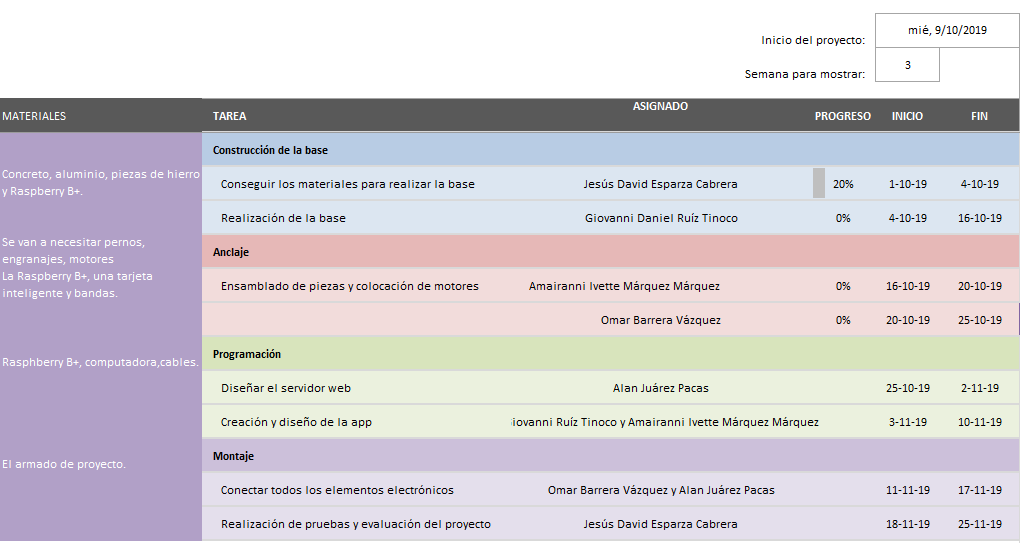
\includegraphics[width=7.11in,height=3.79in]{./media/image2.png}
	\end{Center}
\end{figure}


%%%%%%%%%%%%%%%%%%%% Figure/Image No: 2 Ends here %%%%%%%%%%%%%%%%%%%%

\par


\vspace{\baselineskip}
\textbf{Calendario }\par



%%%%%%%%%%%%%%%%%%%% Figure/Image No: 3 starts here %%%%%%%%%%%%%%%%%%%%

\begin{figure}[H]
	\begin{Center}
		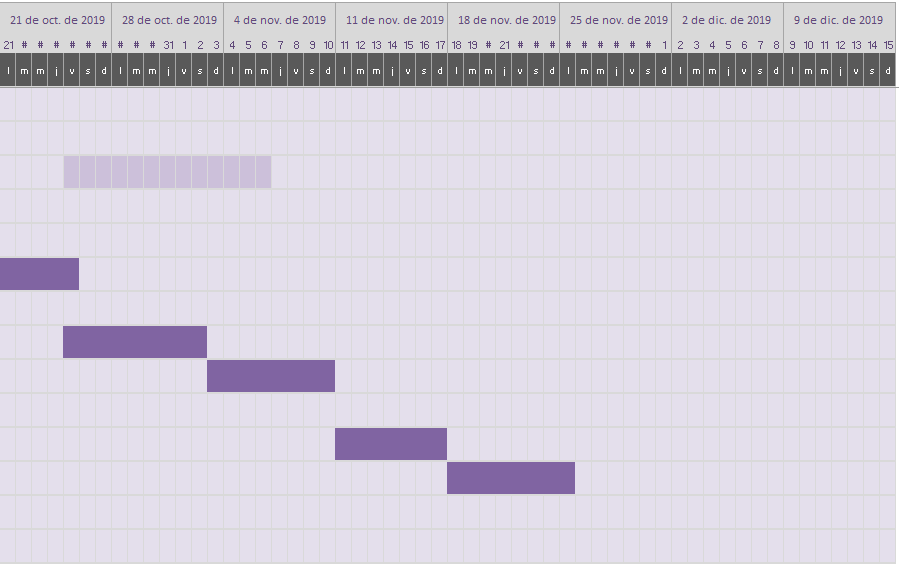
\includegraphics[width=7.18in,height=4.52in]{./media/image3.png}
	\end{Center}
\end{figure}


%%%%%%%%%%%%%%%%%%%% Figure/Image No: 3 Ends here %%%%%%%%%%%%%%%%%%%%

\par


\vspace{\baselineskip}

\vspace{\baselineskip}

\vspace{\baselineskip}

\vspace{\baselineskip}

\vspace{\baselineskip}

\vspace{\baselineskip}

\vspace{\baselineskip}

\vspace{\baselineskip}

\vspace{\baselineskip}

\vspace{\baselineskip}

\vspace{\baselineskip}

\vspace{\baselineskip}

\vspace{\baselineskip}

\vspace{\baselineskip}

\vspace{\baselineskip}
\textbf{Aportación del proyecto en cada una de las asignaturas}\par



%%%%%%%%%%%%%%%%%%%% Table No: 2 starts here %%%%%%%%%%%%%%%%%%%%


\begin{table}[H]
 			\centering
\begin{tabular}{p{1.16in}p{4.5in}}
\hline
%row no:1
\multicolumn{1}{|p{1.16in}}{\Centering {\fontsize{10pt}{12.0pt}\selectfont \textbf{Materias de 4to}}} & 
\multicolumn{1}{|p{4.5in}|}{\Centering {\fontsize{10pt}{12.0pt}\selectfont \textbf{Detalles de la Aportación al proyecto}}} \\
\hhline{--}
%row no:2
\multicolumn{1}{|p{1.16in}}{\Centering {\fontsize{10pt}{12.0pt}\selectfont INGLÉS IV}} & 
\multicolumn{1}{|p{4.5in}|}{{\fontsize{10pt}{12.0pt}\selectfont  }Dado que la búsqueda de Datasheets e investigaciones es indispensable un dominio básico del idioma para así podernos documentarnos en ciertos aspectos como las especificaciones de los fabricantes de algunos materiales.} \\
\hhline{--}
%row no:3
\multicolumn{1}{|p{1.16in}}{\Centering {\fontsize{10pt}{12.0pt}\selectfont ÉTICA PROFESIONAL}} & 
\multicolumn{1}{|p{4.5in}|}{{\fontsize{10pt}{12.0pt}\selectfont  }Dado que la búsqueda de Datasheets e investigaciones es indispensable un dominio básico del idioma para así podernos documentarnos en ciertos aspectos como las especificaciones de los fabricantes de algunos materiales.} \\
\hhline{--}
%row no:4
\multicolumn{1}{|p{1.16in}}{\Centering {\fontsize{10pt}{12.0pt}\selectfont ESTRUCTURA Y PROPIEDADES DE LOS MATERIALES}} & 
\multicolumn{1}{|p{4.5in}|}{Con esta materia podemos tener un criterio más amplio sobre las propiedades necesarias en los materiales que son más convenientes para el uso en nuestro proyecto, tomando en cuenta desde resistencia hasta los costos.} \\
\hhline{--}
%row no:5
\multicolumn{1}{|p{1.16in}}{\Centering {\fontsize{10pt}{12.0pt}\selectfont PROGRAMACIÓN DE PERIFÉRICOS}} & 
\multicolumn{1}{|p{4.5in}|}{En esta aprendemos a configurar los sistemas que vamos a usar y a interconectarlos a través del software que nosotros vamos a desarrollar para ser aplicado en este proyecto. \par } \\
\hhline{--}
%row no:6
\multicolumn{1}{|p{1.16in}}{\Centering {\fontsize{10pt}{12.0pt}\selectfont SISTEMAS ELECTRÓNICOS DE INTERFAZ}} & 
\multicolumn{1}{|p{4.5in}|}{Nos ayuda en la realización del análisis de la automatización necesaria para nuestro proyecto, así como en la definición de procesos y operaciones a automatizar también a efectuar el análisis de la función de entrada como el de las funciones de salida las cuales sea necesario integrar o automatizar en el sistema.} \\
\hhline{--}
%row no:7
\multicolumn{1}{|p{1.16in}}{\Centering {\fontsize{10pt}{12.0pt}\selectfont CONTROLADORES LÓGICOS PROGRAMABLES}} & 
\multicolumn{1}{|p{4.5in}|}{{\fontsize{10pt}{12.0pt}\selectfont  }Con los conocimientos que adquiridos en esta materia podemos aplicar en la fase control para los controladores que usaremos en los motores que moverán el sistema mecánico.} \\
\hhline{--}

\end{tabular}
 \end{table}


%%%%%%%%%%%%%%%%%%%% Table No: 2 ends here %%%%%%%%%%%%%%%%%%%%


\vspace{\baselineskip}
\textbf{Bibliografía }\par

\textit{El informador. (2019). En tres años se duplica robo de motos con violencia en Jalisco. 09/10/19, de El Informador Sitio web: En tres años se duplica robo de motos con violencia en Jalisco}\par

Notimex. (2019).Estas son las motocicletas más robadas del país 09/10/19, de El universal Sitio web: \href{https://www.eluniversal.com.mx/cartera/economia/estas-son-las-motocicletas-mas-robadas-en-el-pais}{https://www.eluniversal.com.mx/cartera/economia/estas-son-las-motocicletas-mas-robadas-en-el-pais}\par

Jorge Martínez. (2018). Roban 6 motocicletas al día en Jalisco: FGE. 09/10/19, de Milenio Sitio web: \href{https://www.milenio.com/politica/comunidad/roban-6-motocicletas-al-dia-en-jalisco-fge}{https://www.milenio.com/politica/comunidad/roban-6-motocicletas-al-dia-en-jalisco-fge}\par


\vspace{\baselineskip}

\printbibliography
\end{document}